\documentclass{beamer}
\usepackage[latin1]{inputenc}
%\usetheme{Montpellier}
%\usetheme{Boadilla}
%\usecolortheme[RGB={204,51,255}]{structure}
%\usecolortheme[named=purple]{structure}
\usecolortheme[RGB={128,62,62}]{structure}
%\definecolor{dark}{rgb}{0.3,0.15,0.3}
%\definecolor{light}{rgb}{0.8,0.6,0.8}
%\definecolor{reddish}{rgb}{.5,0.15,0.15}
\definecolor{dark}{rgb}{0.5,0.3,0.4}
%\definecolor{light}{rgb}{0.8,0.6,0.8}
\definecolor{reddish}{rgb}{.7,0.25,0.25}
\definecolor{greenish}{rgb}{.25,0.7,0.25}
\definecolor{blueish}{rgb}{.25,0.25,0.7}
\definecolor{purple}{rgb}{.5,0.0,0.5}
\usepackage{graphicx}
\usepackage{pstricks}

\usepackage{amssymb}

\usepackage{amsmath}
\setbeamertemplate{navigation symbols}{}

\newcommand{\crish}{\color{reddish}}
\newcommand{\cbla}{\color{black}}
\newcommand{\cred}{\color{red}}
\newcommand{\cblu}{\color{blue}}

\newcommand{\sm}{\color{reddish}$}
\newcommand{\fm}{$\color{black}}
\usepackage{tikz}
\usetikzlibrary{arrows,decorations.markings,positioning}
\usetikzlibrary{calc,fit,shapes, backgrounds} 

\usepackage{epstopdf}
\title{Lecture 5: Conditional Probability}
\author{COMS10014 Mathematics for Computer Science A}
\institute{\texttt{cs-uob.github.io/COMS10014/ and github.com/coms10011/2020\_21}}
\date{November 2020}
\begin{document}
\maketitle
\begin{frame}{The Nobel Prize for Literature is sexist.}
  \begin{itemize}
  \item 117 individuals have won the Nobel Prize for Literature.
  \item Sixteen woman have won.
  \item \crish$16/117\approx 0.14$\cbla{}.
  \end{itemize}
\crish  $$P(\mbox{woman})=0.14$$\cbla
\end{frame}

\begin{frame}{The Booker Prize is less sexist?}
  \begin{itemize}
  \item Seven people have won both the Booker Prize and the Nobel Prize for Literature.
  \item Of that seven three were women.
  \item \crish$3/7\approx 0.43$\cbla.
  \end{itemize}
\end{frame}


\begin{frame}{Doris Lessing / Alice Munro / Nadine Gordimer}
     \begin{center}
    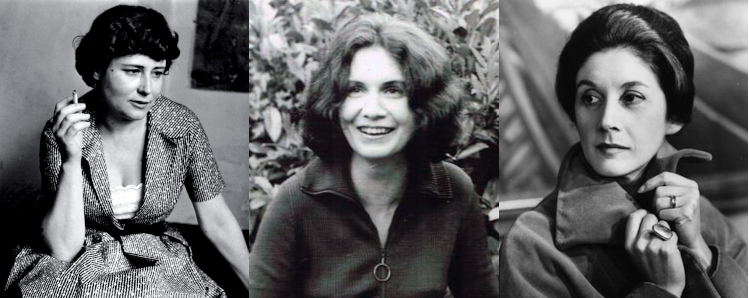
\includegraphics[width=8cm]{writers.png}
    \end{center}
\end{frame}


\begin{frame}{Nobel Prize probabilities}
\begin{center}
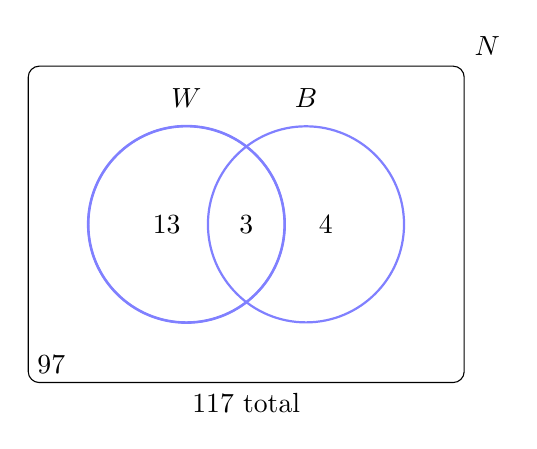
\begin{tikzpicture}
\colorlet{circle edge}{blue!50}
\colorlet{circle area}{blue!20}
\tikzset{
     filled/.style={fill=circle area, thick,inner sep=0pt}, 
     outline/.style={draw=circle edge, thick,inner sep=0pt}}

% The circles
\node (firstcircle)  [circle,text width=2.5cm, outline] {};
\node (secondcircle) [circle, right=-1cm of firstcircle,white,text width=2.5cm,outline] {};
\draw [outline] (firstcircle) circle (1.25cm);



\node at ([yshift=0.35cm]firstcircle.north){$W$};
\node at ([yshift=0.35cm]secondcircle.north){$B$};

% The labels
\node at ([xshift=-0.25cm]firstcircle) {$13$};
\node at ([xshift= 0.25cm]secondcircle) {$4$};
\node at ($(firstcircle)!0.5!(secondcircle)$) {3};

% The rectangle and labels

\node (box) [fit=(firstcircle)(secondcircle), inner sep=0.75cm,draw,rounded corners] {};

\node at (box.north) [anchor=north] {};
\node at (box.south west) [anchor=south west] {97};
\node at (box.south) [anchor=north] {117 total};
\node at (box.north east) [anchor=south west] {$N$};
\end{tikzpicture}
\end{center}
\end{frame}


\begin{frame}{Nobel Prize probabilities - woman}
\begin{center}
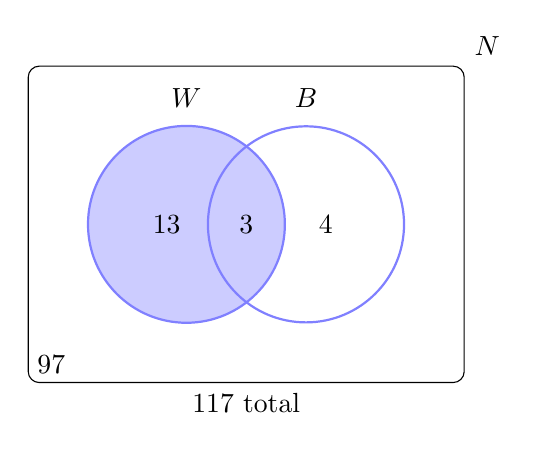
\begin{tikzpicture}
\colorlet{circle edge}{blue!50}
\colorlet{circle area}{blue!20}
\tikzset{
     filled/.style={fill=circle area, thick,inner sep=0pt}, 
     outline/.style={draw=circle edge, thick,inner sep=0pt}}

% The circles
\node (firstcircle)  [circle,text width=2.5cm, filled] {};
\node (secondcircle) [circle, right=-1cm of firstcircle,white,text width=2.5cm,outline] {};
\draw [outline] (firstcircle) circle (1.25cm);



\node at ([yshift=0.35cm]firstcircle.north){$W$};
\node at ([yshift=0.35cm]secondcircle.north){$B$};

% The labels
\node at ([xshift=-0.25cm]firstcircle) {$13$};
\node at ([xshift= 0.25cm]secondcircle) {$4$};
\node at ($(firstcircle)!0.5!(secondcircle)$) {3};

% The rectangle and labels

\node (box) [fit=(firstcircle)(secondcircle), inner sep=0.75cm,draw,rounded corners] {};

\node at (box.north) [anchor=north] {};
\node at (box.south west) [anchor=south west] {97};
\node at (box.south) [anchor=north] {117 total};
\node at (box.north east) [anchor=south west] {$N$};
\end{tikzpicture}
\end{center}
\crish$$P(W)=16/117\approx 0.14$$\cbla
\end{frame}


\begin{frame}{Nobel Prize probabilities - woman or booker}
\begin{center}
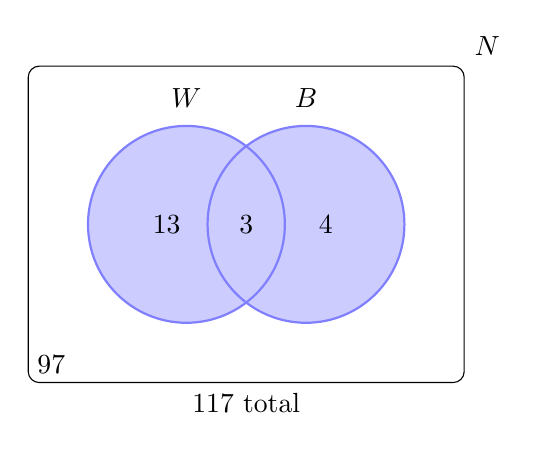
\begin{tikzpicture}
\colorlet{circle edge}{blue!50}
\colorlet{circle area}{blue!20}
\tikzset{
     filled/.style={fill=circle area, thick,inner sep=0pt}, 
     outline/.style={draw=circle edge, thick,inner sep=0pt}}

% The circles
\node (firstcircle)  [circle,text width=2.5cm, filled] {};
\node (secondcircle) [circle, right=-1cm of firstcircle,white,text width=2.5cm,filled] {};
\draw [outline] (firstcircle) circle (1.25cm);
\draw [outline] (secondcircle) circle (1.25cm);



\node at ([yshift=0.35cm]firstcircle.north){$W$};
\node at ([yshift=0.35cm]secondcircle.north){$B$};

% The labels
\node at ([xshift=-0.25cm]firstcircle) {$13$};
\node at ([xshift= 0.25cm]secondcircle) {$4$};
\node at ($(firstcircle)!0.5!(secondcircle)$) {3};

% The rectangle and labels

\node (box) [fit=(firstcircle)(secondcircle), inner sep=0.75cm,draw,rounded corners] {};

\node at (box.north) [anchor=north] {};
\node at (box.south west) [anchor=south west] {97};
\node at (box.south) [anchor=north] {117 total};
\node at (box.north east) [anchor=south west] {$N$};
\end{tikzpicture}
\end{center}
\crish$$P(W\cup B)=20/117\approx 0.17$$\cbla
\end{frame}


\begin{frame}{Nobel Prize probabilities - woman and booker}
\begin{center}
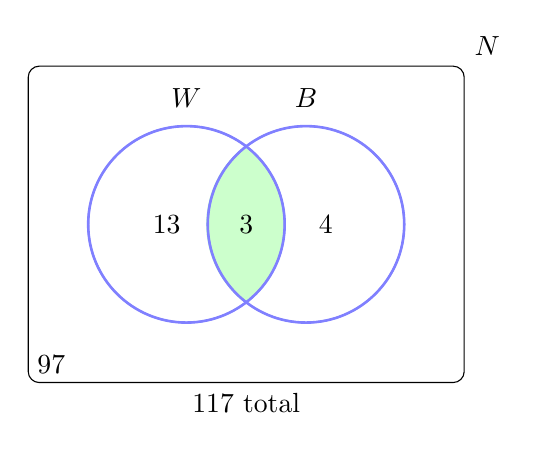
\begin{tikzpicture}
\colorlet{circle edge}{blue!50}
\colorlet{circle area}{blue!20}
\tikzset{
     filled/.style={fill=circle area, thick,inner sep=0pt}, 
     outline/.style={draw=circle edge, thick,inner sep=0pt}}


%I know what a hack this is and I am sorry
\def\acircle{(0.0,0) circle (1.25cm)};
\def\bcircle{(1.5,0) circle (1.25cm)};


\begin{scope}
  \clip \acircle;
  \fill[green!20] \bcircle;
\end{scope}


% The circles
\node (firstcircle)  [circle,text width=2.5cm, outline] {};
\node (secondcircle) [circle, right=-1cm of firstcircle,white,text width=2.5cm,outline] {};
\draw [outline] (firstcircle) circle (1.25cm);
\draw [outline] (secondcircle) circle (1.25cm);


\node at ([yshift=0.35cm]firstcircle.north){$W$};
\node at ([yshift=0.35cm]secondcircle.north){$B$};

% The labels
\node at ([xshift=-0.25cm]firstcircle) {$13$};
\node at ([xshift= 0.25cm]secondcircle) {$4$};
\node at ($(firstcircle)!0.5!(secondcircle)$) {3};

% The rectangle and labels

\node (box) [fit=(firstcircle)(secondcircle), inner sep=0.75cm,draw,rounded corners] {};

\node at (box.north) [anchor=north] {};
\node at (box.south west) [anchor=south west] {97};
\node at (box.south) [anchor=north] {117 total};
\node at (box.north east) [anchor=south west] {$N$};
\end{tikzpicture}
\end{center}
\crish$$P(W\cap B)=3/117\approx 0.03$$\cbla
\end{frame}


\begin{frame}{Nobel Prize probabilities - woman given booker}
\begin{center}
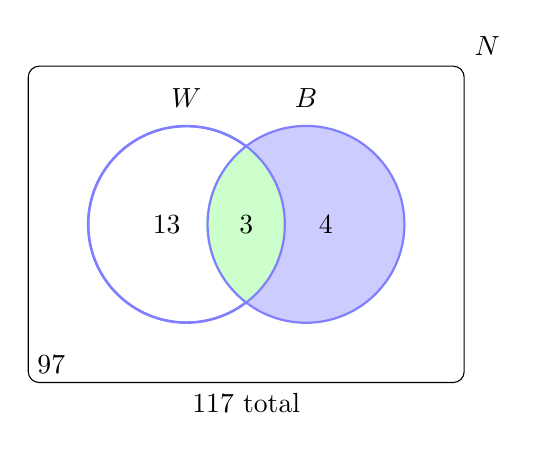
\begin{tikzpicture}
\colorlet{circle edge}{blue!50}
\colorlet{circle area}{blue!20}
\tikzset{
     filled/.style={fill=circle area, thick,inner sep=0pt}, 
     outline/.style={draw=circle edge, thick,inner sep=0pt}}


%I know what a hack this is and I am sorry
\def\acircle{(0.0,0) circle (1.25cm)};
\def\bcircle{(1.5,0) circle (1.25cm)};



% The circles
\node (firstcircle)  [circle,text width=2.5cm, outline] {};
\node (secondcircle) [circle, right=-1cm of firstcircle,white,text width=2.5cm,filled] {};

\begin{scope}
  \clip \acircle;
  \fill[green!20] \bcircle;
\end{scope}


\draw [outline] (firstcircle) circle (1.25cm);
\draw [outline] (secondcircle) circle (1.25cm);


\node at ([yshift=0.35cm]firstcircle.north){$W$};
\node at ([yshift=0.35cm]secondcircle.north){$B$};

% The labels
\node at ([xshift=-0.25cm]firstcircle) {$13$};
\node at ([xshift= 0.25cm]secondcircle) {$4$};
\node at ($(firstcircle)!0.5!(secondcircle)$) {3};

% The rectangle and labels

\node (box) [fit=(firstcircle)(secondcircle), inner sep=0.75cm,draw,rounded corners] {};

\node at (box.north) [anchor=north] {};
\node at (box.south west) [anchor=south west] {97};
\node at (box.south) [anchor=north] {117 total};
\node at (box.north east) [anchor=south west] {$N$};
\end{tikzpicture}
\end{center}
\crish$$P(W\mbox{ given }B)=3/7\approx 0.43$$\cbla
\end{frame}

\begin{frame}{Conditional probability}
  If we have two events \crish$A$\cbla{} and \crish$B$\cbla{} then
  \crish$$
  P(A|B)=\frac{P(A\cap B)}{P(B)}
  $$\cbla{}
  is the probability of \crish$A$\cbla{} given \crish$B$\cbla{}. This is the \textbf{conditional probability}.
\end{frame}


\begin{frame}{Nobel Prize probabilities - woman given booker}
\begin{center}
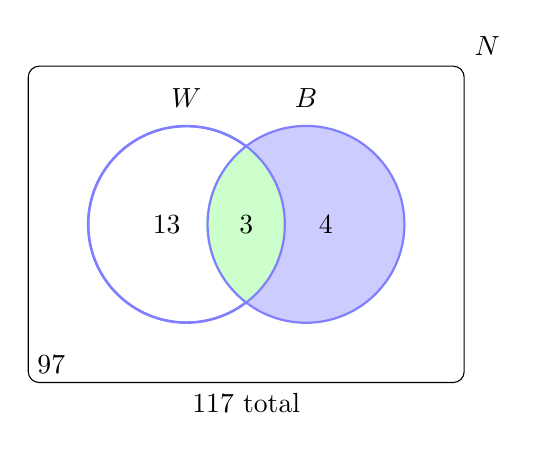
\begin{tikzpicture}
\colorlet{circle edge}{blue!50}
\colorlet{circle area}{blue!20}
\tikzset{
     filled/.style={fill=circle area, thick,inner sep=0pt}, 
     outline/.style={draw=circle edge, thick,inner sep=0pt}}


%I know what a hack this is and I am sorry
\def\acircle{(0.0,0) circle (1.25cm)};
\def\bcircle{(1.5,0) circle (1.25cm)};



% The circles
\node (firstcircle)  [circle,text width=2.5cm, outline] {};
\node (secondcircle) [circle, right=-1cm of firstcircle,white,text width=2.5cm,filled] {};

\begin{scope}
  \clip \acircle;
  \fill[green!20] \bcircle;
\end{scope}


\draw [outline] (firstcircle) circle (1.25cm);
\draw [outline] (secondcircle) circle (1.25cm);


\node at ([yshift=0.35cm]firstcircle.north){$W$};
\node at ([yshift=0.35cm]secondcircle.north){$B$};

% The labels
\node at ([xshift=-0.25cm]firstcircle) {$13$};
\node at ([xshift= 0.25cm]secondcircle) {$4$};
\node at ($(firstcircle)!0.5!(secondcircle)$) {3};

% The rectangle and labels

\node (box) [fit=(firstcircle)(secondcircle), inner sep=0.75cm,draw,rounded corners] {};

\node at (box.north) [anchor=north] {};
\node at (box.south west) [anchor=south west] {97};
\node at (box.south) [anchor=north] {117 total};
\node at (box.north east) [anchor=south west] {$N$};
\end{tikzpicture}
\end{center}
\crish$$P(W|B)=\frac{P(W\cap B)}{P(B)} = \frac{3/117}{7/117} = \frac{3}{7}\approx 0.43$$\cbla
\end{frame}



\begin{frame}{Conditional probability}
  \crish$$
  P(A\cap B)=P(A|B)P(B)
  $$\cbla{}
means the probability of \crish$A$\cbla{} \textbf{and} \crish$B$\cbla{} is the probability of \crish$B$\cbla{} multiplied by the probability of \crish$A$\cbla{} \textbf{given} \crish$B$\cbla{}.
\end{frame}




\end{document}
